\documentclass[11pt,letterpaper,oneside,openany]{report}

% -----------------------------------------------------------------------------
% Manual de usuario de HCNet Transport 2.0.0
% Compilacion recomendada: pdflatex -> makeindex -> pdflatex -> pdflatex
% -----------------------------------------------------------------------------
\usepackage[utf8]{inputenc}
\usepackage[T1]{fontenc}
\usepackage{lmodern}
\usepackage[provide=*,spanish]{babel}
\usepackage[letterpaper,top=2.05cm,bottom=2.05cm,left=2.15cm,right=2.15cm,
            headheight=16pt,headsep=0.55cm,footskip=0.8cm]{geometry}
\usepackage[table]{xcolor}
\usepackage{graphicx}
\usepackage{amsmath,amssymb}
\usepackage{booktabs,longtable,tabularx,array}
\usepackage{enumitem}
\usepackage{listings}
\usepackage[most]{tcolorbox}
\usepackage{titlesec}
\usepackage{fancyhdr}
\usepackage{caption}
\usepackage{float}
\usepackage{microtype}
\usepackage{makeidx}
\usepackage[hidelinks]{hyperref}

\hypersetup{
  pdftitle={Manual de usuario de HCNet Transport 2.0.0},
  pdfauthor={Héctor Alonso Benítez García},
  pdfsubject={Operación y fundamento metodológico de HCNet Transport},
  pdfkeywords={HCNet, HCM, intersecciones semaforizadas, capacidad, nivel de servicio}
}

\graphicspath{{assets/}}
\makeindex

% --- Identidad documental ----------------------------------------------------
\newcommand{\softwareName}{HCNet Transport}
\newcommand{\softwareVersion}{2.0.0}
\newcommand{\manualVersion}{1.0}
\newcommand{\developerName}{Héctor Alonso Benítez García}
\newcommand{\repositoryURL}{https://github.com/VanLinux/hcnet-transport}
\newcommand{\releaseDate}{septiembre de 2026}

% --- Paleta profesional compatible con la interfaz neutral ------------------
\definecolor{hcBlack}{HTML}{20242A}
\definecolor{hcGraphite}{HTML}{3F444B}
\definecolor{hcGray}{HTML}{5F6368}
\definecolor{hcLine}{HTML}{DADCE0}
\definecolor{hcPale}{HTML}{F1F3F4}
\definecolor{hcPaper}{HTML}{FAFAFA}
\definecolor{hcAccent}{HTML}{405D66}
\definecolor{hcGreen}{HTML}{176B45}
\definecolor{hcGreenPale}{HTML}{EAF4EE}
\definecolor{hcAmber}{HTML}{8A5A16}
\definecolor{hcAmberPale}{HTML}{FBF4E8}
\definecolor{hcRed}{HTML}{9F2D2D}
\definecolor{hcRedPale}{HTML}{F9ECEC}

% --- Tipografia y ritmo ------------------------------------------------------
\setlength{\parindent}{0pt}
\setlength{\parskip}{5pt plus 1pt minus 1pt}
\setlength{\emergencystretch}{3em}
\renewcommand{\arraystretch}{1.18}
\setlist[itemize]{leftmargin=1.25em,itemsep=2pt,topsep=4pt}
\setlist[enumerate]{leftmargin=1.55em,itemsep=3pt,topsep=4pt}
\captionsetup{font=small,labelfont={bf,color=hcGraphite},textfont={color=hcGray},
              skip=5pt}
\newcolumntype{Y}{>{\raggedright\arraybackslash}X}
\newcolumntype{C}[1]{>{\centering\arraybackslash}p{#1}}
\newcolumntype{R}[1]{>{\raggedleft\arraybackslash}p{#1}}

% --- Titulos -----------------------------------------------------------------
\titleformat{\chapter}[display]
  {\normalfont\color{hcBlack}}
  {\filleft\Large\bfseries\textcolor{hcGray}{CAPÍTULO \thechapter}}
  {0.35ex}
  {\titlerule[1.1pt]\vspace{0.8ex}\Huge\bfseries}
\titlespacing*{\chapter}{0pt}{-16pt}{22pt}
\titleformat{\section}{\Large\bfseries\color{hcBlack}}
  {\thesection}{0.65em}{}
\titleformat{\subsection}{\large\bfseries\color{hcGraphite}}
  {\thesubsection}{0.65em}{}

% --- Encabezados y pies ------------------------------------------------------
\pagestyle{fancy}
\fancyhf{}
\fancyhead[L]{\small\textcolor{hcGray}{\softwareName\ \softwareVersion}}
\fancyhead[R]{\small\textcolor{hcGray}{Manual de usuario}}
\fancyfoot[L]{\small\textcolor{hcGray}{Edición \manualVersion}}
\fancyfoot[R]{\small\textcolor{hcGray}{\thepage}}
\renewcommand{\headrulewidth}{0.35pt}
\renewcommand{\footrulewidth}{0pt}
\fancypagestyle{plain}{
  \fancyhf{}
  \fancyfoot[L]{\small\textcolor{hcGray}{\softwareName\ - Manual de usuario}}
  \fancyfoot[R]{\small\textcolor{hcGray}{\thepage}}
  \renewcommand{\headrulewidth}{0pt}
}

% --- Recuadros ---------------------------------------------------------------
\newtcolorbox{keybox}[1][Punto clave]{
  enhanced,breakable,colback=hcPale,colframe=hcAccent,coltitle=white,
  fonttitle=\bfseries,title=#1,boxrule=0.7pt,arc=1.2mm,
  left=3mm,right=3mm,top=2mm,bottom=2mm,
  attach boxed title to top left={xshift=3mm,yshift*=-2mm},
  boxed title style={colback=hcAccent,colframe=hcAccent,arc=1mm}
}
\newtcolorbox{procedurebox}[1][Procedimiento]{
  enhanced,breakable,colback=hcPaper,colframe=hcGraphite,coltitle=white,
  fonttitle=\bfseries,title=#1,boxrule=0.7pt,arc=1.2mm,
  left=3mm,right=3mm,top=2mm,bottom=2mm,
  attach boxed title to top left={xshift=3mm,yshift*=-2mm},
  boxed title style={colback=hcGraphite,colframe=hcGraphite,arc=1mm}
}
\newtcolorbox{tipbox}[1][Buena práctica]{
  enhanced,breakable,colback=hcGreenPale,colframe=hcGreen,coltitle=white,
  fonttitle=\bfseries,title=#1,boxrule=0.7pt,arc=1.2mm,
  left=3mm,right=3mm,top=2mm,bottom=2mm,
  attach boxed title to top left={xshift=3mm,yshift*=-2mm},
  boxed title style={colback=hcGreen,colframe=hcGreen,arc=1mm}
}
\newtcolorbox{warningbox}[1][Advertencia]{
  enhanced,breakable,colback=hcAmberPale,colframe=hcAmber,coltitle=white,
  fonttitle=\bfseries,title=#1,boxrule=0.7pt,arc=1.2mm,
  left=3mm,right=3mm,top=2mm,bottom=2mm,
  attach boxed title to top left={xshift=3mm,yshift*=-2mm},
  boxed title style={colback=hcAmber,colframe=hcAmber,arc=1mm}
}
\newtcolorbox{limitbox}[1][Límite de alcance]{
  enhanced,breakable,colback=hcRedPale,colframe=hcRed,coltitle=white,
  fonttitle=\bfseries,title=#1,boxrule=0.7pt,arc=1.2mm,
  left=3mm,right=3mm,top=2mm,bottom=2mm,
  attach boxed title to top left={xshift=3mm,yshift*=-2mm},
  boxed title style={colback=hcRed,colframe=hcRed,arc=1mm}
}
\newtcolorbox{equationbox}[1][Implementación en HCNet]{
  enhanced,breakable,colback=hcPaper,colframe=hcLine,coltitle=hcBlack,
  fonttitle=\bfseries,title=#1,boxrule=0.6pt,arc=1mm,
  borderline west={3pt}{0pt}{hcAccent},left=4mm,right=3mm,top=2mm,bottom=2mm
}

% --- Listados de terminal ----------------------------------------------------
\lstdefinestyle{hcnetterminal}{
  basicstyle=\ttfamily\small,
  backgroundcolor=\color{hcBlack},
  basicstyle=\ttfamily\small\color{white},
  keywordstyle=\color{white}\bfseries,
  commentstyle=\color{hcLine},
  frame=single,rulecolor=\color{hcGraphite},framerule=0.4pt,
  xleftmargin=0.6em,xrightmargin=0.6em,aboveskip=6pt,belowskip=6pt,
  breaklines=true,showstringspaces=false,columns=fullflexible,
  keepspaces=true
}
\lstset{style=hcnetterminal}

% --- Nombres en espanol ------------------------------------------------------
\renewcommand{\contentsname}{Índice general}
\renewcommand{\listfigurename}{Índice de figuras}
\renewcommand{\listtablename}{Índice de tablas}
\renewcommand{\bibname}{Referencias}
\renewcommand{\indexname}{Índice alfabético}
\addto\captionsspanish{
  \renewcommand{\contentsname}{Índice general}
  \renewcommand{\listfigurename}{Índice de figuras}
  \renewcommand{\listtablename}{Índice de cuadros}
  \renewcommand{\bibname}{Referencias}
}

\begin{document}
\hypersetup{pageanchor=false}

% =============================================================================
% Portada
% =============================================================================
\begin{titlepage}
  \thispagestyle{empty}
  \color{hcBlack}
  \vspace*{0.8cm}
  \begin{tcolorbox}[
    colback=hcBlack,colframe=hcBlack,arc=1.5mm,boxrule=0pt,
    left=8mm,right=8mm,top=9mm,bottom=9mm]
    \color{white}
    {\fontsize{33}{37}\selectfont\bfseries HCNet Transport\par}
    \vspace{1.5mm}
    {\Large Análisis de intersecciones semaforizadas aisladas\par}
  \end{tcolorbox}

  \vspace{1.5cm}
  {\fontsize{29}{33}\selectfont\bfseries Manual de usuario\par}
  \vspace{0.3cm}
  {\Large Edición \manualVersion\ para HCNet \softwareVersion\par}
  \vspace{0.7cm}
  \textcolor{hcAccent}{\rule{\textwidth}{1.4pt}}

  \vspace{1.0cm}
  \begin{keybox}[Finalidad del documento]
  Guía para instalar, configurar, operar y revisar HCNet Transport en Linux.
  Incluye la base matemática implementada, criterios de nivel de servicio,
  validación de datos, exportación de resultados y un caso demostrativo
  reproducible.
  \end{keybox}

  \vfill
  \begin{tabularx}{\textwidth}{@{}p{4.2cm}Y@{}}
    \textbf{Desarrollador} & \developerName \\
    \textbf{Licencia del software} & GNU General Public License v3.0 only \\
    \textbf{Plataforma de esta edición} & Linux \\
    \textbf{Fecha de publicación} & \releaseDate \\
    \textbf{Repositorio oficial} & \href{\repositoryURL}{github.com/VanLinux/hcnet-transport} \\
  \end{tabularx}

  \vspace{0.8cm}
  {\small\textcolor{hcGray}{Documento técnico de usuario. Tamaño de página: carta.}}
\end{titlepage}

% =============================================================================
% Preliminares
% =============================================================================
\hypersetup{pageanchor=true}
\pagenumbering{roman}

\chapter*{Control del documento}
\addcontentsline{toc}{chapter}{Control del documento}

\begin{tabularx}{\textwidth}{@{}p{4.6cm}Y@{}}
\toprule
\rowcolor{hcPale}
\textbf{Elemento} & \textbf{Identificación} \\
\midrule
Título & Manual de usuario de HCNet Transport \\
Edición del manual & \manualVersion \\
Versión documentada del software & \softwareVersion \\
Autor y desarrollador & \developerName \\
Sistema operativo objetivo & Distribuciones Linux de escritorio \\
Licencia del software & GNU GPL v3.0 only \\
Idioma & Español \\
Estado & Edición inicial para revisión de interfaz y operación \\
\bottomrule
\end{tabularx}

\section*{Registro de revisiones}
\phantomsection
\addcontentsline{toc}{section}{Registro de revisiones}

\begin{tabularx}{\textwidth}{@{}C{1.8cm}C{2.7cm}Y@{}}
\toprule
\rowcolor{hcPale}
\textbf{Edición} & \textbf{Fecha} & \textbf{Descripción} \\
\midrule
1.0 & Septiembre de 2026 & Primera edición integral para HCNet Transport
2.0.0; instalación en Linux, operación, metodología, reportes y caso de prueba. \\
\bottomrule
\end{tabularx}

\begin{warningbox}[Responsabilidad profesional]
HCNet Transport es una aplicación educativa e independiente. No está afiliada,
certificada ni respaldada por Transportation Research Board (TRB), National
Academies, McTrans Center o Highway Capacity Software (HCS). Antes de utilizar
resultados en un dictamen, proyecto ejecutivo o estudio contractual, el analista
debe comprobar los datos, la aplicabilidad del modelo y la consistencia con una
fuente metodológica autorizada.
\end{warningbox}

\section*{Licencia y atribución}
\phantomsection
\addcontentsline{toc}{section}{Licencia y atribución}

El código fuente de \softwareName\ se distribuye bajo la licencia
\textit{GNU General Public License v3.0 only}. La licencia permite estudiar,
modificar y redistribuir el programa conforme a sus términos. El nombre HCM y
las publicaciones asociadas pertenecen a sus respectivos titulares; este manual
no reproduce tablas propietarias ni sustituye la consulta legítima del HCM.

\begin{tipbox}[Cómo citar el software]
Para trabajos académicos o técnicos, utilice el archivo \texttt{CITATION.cff}
del repositorio. Registre siempre la versión de HCNet, la fecha del análisis y
el nombre del analista para conservar trazabilidad.
\end{tipbox}

\clearpage
\tableofcontents
\clearpage
\listoffigures
\addcontentsline{toc}{chapter}{Índice de figuras}
\clearpage
\listoftables
\addcontentsline{toc}{chapter}{Índice de tablas}
\clearpage

\pagenumbering{arabic}

% =============================================================================
\chapter{Introducción y alcance}
% =============================================================================

\section{Propósito del manual}

Este manual explica el uso completo de \softwareName\ \softwareVersion\ para
analizar la capacidad, el grado de saturación, la demora de control y el nivel de
servicio de grupos de carriles en una intersección semaforizada aislada.
\index{manual!propósito}

El documento está dirigido a profesionales de tránsito, docentes, investigadores
y estudiantes con conocimientos de ingeniería de transporte. Se presupone que
el usuario puede identificar grupos de carriles, obtener volúmenes de demanda,
interpretar un plan semafórico y seleccionar parámetros de ajuste con respaldo
técnico.

\section{Alcance funcional de HCNet}

La versión documentada trabaja con las siguientes condiciones:

\begin{itemize}
  \item intersecciones semaforizadas aisladas;
  \item control de tiempo fijo y longitud de ciclo común;
  \item demanda estacionaria durante un periodo de análisis definido;
  \item cálculo independiente por grupo de carriles;
  \item estimación de flujo de saturación ajustado, capacidad, relación
        demanda-capacidad, demora de control y nivel de servicio;
  \item consolidación de la demora de la intersección mediante ponderación por
        flujo de demanda ajustado;
  \item guardado del proyecto, exportación tabular CSV y memoria técnica en
        código fuente LaTeX.
\end{itemize}

\begin{limitbox}
La versión \softwareVersion\ no modela internamente coordinación de corredores,
control actuado, tránsito peatonal o ciclista, glorietas, accesos no controlados,
segmentos viales, autopistas, calibración automática para México, asignación
automática de carriles compartidos ni cola percentil 95. La demanda residual que
muestra la aplicación es un indicador diagnóstico; no es una estimación HCM de
cola percentil 95.
\end{limitbox}

\section{Secuencia general de trabajo}

\begin{procedurebox}[Flujo recomendado]
\begin{enumerate}
  \item Identifique el proyecto, la ubicación, el analista, la fecha y el periodo
        de análisis.
  \item Defina cada grupo de carriles con sus volúmenes, geometría, tiempos y
        factores de ajuste.
  \item Revise los diagnósticos automáticos y corrija los errores de entrada.
  \item Ejecute el cálculo y examine el grupo crítico, la demora, el grado de
        saturación y el nivel de servicio.
  \item Consulte la memoria de cálculo por grupo.
  \item Guarde el proyecto y exporte los resultados CSV y el reporte LaTeX.
  \item Documente supuestos, fuentes y decisiones de ingeniería fuera y dentro
        del proyecto.
\end{enumerate}
\end{procedurebox}

\section{Convenciones usadas en este documento}

\begin{tabularx}{\textwidth}{@{}p{3.2cm}Y@{}}
\toprule
\rowcolor{hcPale}
\textbf{Convención} & \textbf{Significado} \\
\midrule
Texto en \textbf{negritas} & Nombre de una pestaña, botón, menú o acción. \\
\texttt{Monoespaciado} & Comando de terminal, nombre de archivo o extensión. \\
Recuadro gris azulado & Concepto esencial o decisión operativa. \\
Recuadro verde & Buena práctica para mejorar la trazabilidad. \\
Recuadro ámbar & Advertencia que exige revisión del analista. \\
Recuadro rojo & Restricción del modelo o riesgo de interpretación. \\
\bottomrule
\end{tabularx}

\begin{figure}[H]
  \centering
  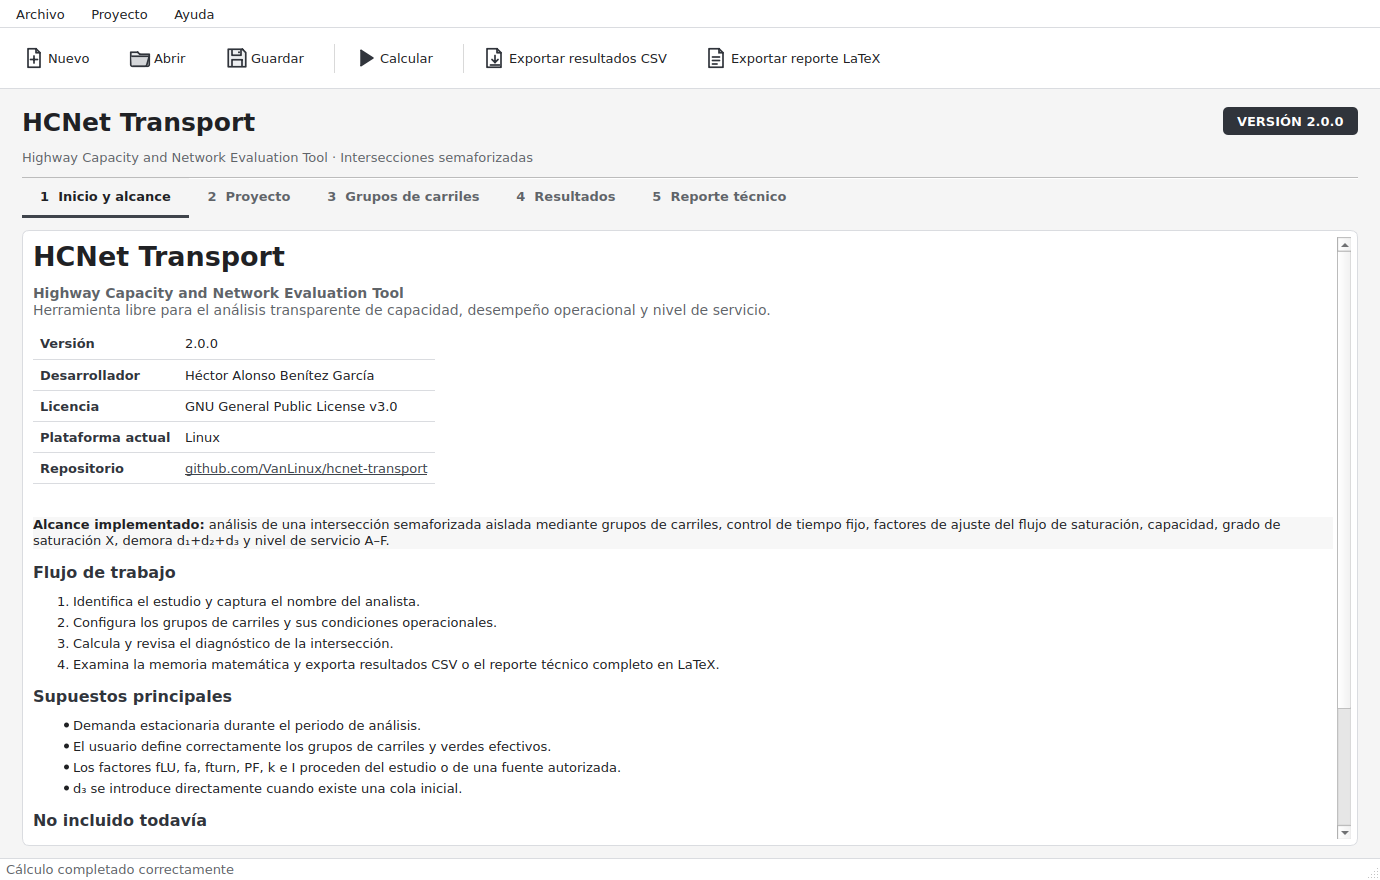
\includegraphics[width=0.98\textwidth]{01_inicio_alcance.png}
  \caption{Pestaña inicial con propósito, flujo de trabajo, alcance y licencia.}
  \label{fig:inicio}
\end{figure}

La pestaña \textbf{Inicio y alcance}, mostrada en la figura~\ref{fig:inicio}, es
el punto de entrada de la aplicación. Se recomienda leerla antes de iniciar el
primer proyecto.\index{alcance}\index{licencia}

% =============================================================================
\chapter{Instalación y puesta en marcha en Linux}
% =============================================================================

\section{Requisitos}

\begin{itemize}
  \item distribución Linux con entorno gráfico de escritorio;
  \item Python 3.11 o posterior;
  \item \texttt{pip} y soporte para entornos virtuales;
  \item acceso al repositorio oficial durante la instalación;
  \item bibliotecas de escritorio requeridas por Qt/PySide6.
\end{itemize}

\begin{keybox}[Aislamiento del entorno]
Instale HCNet dentro de un entorno virtual \texttt{.venv}. Esta práctica evita
mezclar sus dependencias con los paquetes del sistema y facilita reproducir la
instalación.\index{entorno virtual}
\end{keybox}

\section{Instalación en Fedora}

Abra una terminal y ejecute:

\begin{lstlisting}
sudo dnf install python3 python3-pip
git clone https://github.com/VanLinux/hcnet-transport.git
cd hcnet-transport
python3 -m venv .venv
source .venv/bin/activate
python -m pip install --upgrade pip
python -m pip install -e ".[dev]"
hcnet
\end{lstlisting}

\section{Instalación en Ubuntu o Debian}

\begin{lstlisting}
sudo apt install python3 python3-venv python3-pip libxcb-cursor0
git clone https://github.com/VanLinux/hcnet-transport.git
cd hcnet-transport
python3 -m venv .venv
source .venv/bin/activate
python -m pip install --upgrade pip
python -m pip install -e ".[dev]"
hcnet
\end{lstlisting}

\section{Inicios posteriores}

Si el repositorio se encuentra en \texttt{\textasciitilde/hcnet-transport}:

\begin{lstlisting}
cd ~/hcnet-transport
source .venv/bin/activate
hcnet
\end{lstlisting}

Al terminar la sesión puede desactivar el entorno:

\begin{lstlisting}
deactivate
\end{lstlisting}

\section{Comprobación de la instalación}

La instalación es satisfactoria cuando aparece la ventana principal, se muestra
la pestaña \textbf{Inicio y alcance} y el título de la ventana identifica la
versión 2.0.0. Para verificar además el núcleo de cálculo y la lectura de archivos,
ejecute la batería de pruebas desde el directorio del proyecto:

\begin{lstlisting}
pytest
\end{lstlisting}

\begin{tipbox}
Conserve el entorno virtual activo durante toda la sesión. Si la orden
\texttt{hcnet} no existe, verifique primero que el indicador del entorno
\texttt{(.venv)} aparezca en la terminal y repita la instalación editable.
\end{tipbox}

% =============================================================================
\chapter{Interfaz y navegación}
% =============================================================================

\section{Organización de la ventana principal}

La interfaz está organizada de izquierda a derecha según el flujo de análisis.
La tabla~\ref{tab:pestanas} resume las cinco pestañas.

\begin{table}[H]
\centering
\caption{Pestañas de la interfaz principal.}
\label{tab:pestanas}
\begin{tabularx}{\textwidth}{@{}C{1.3cm}p{3.3cm}Y@{}}
\toprule
\rowcolor{hcPale}
\textbf{Orden} & \textbf{Pestaña} & \textbf{Función} \\
\midrule
1 & Inicio y alcance & Presenta el propósito, los límites metodológicos, la
licencia y la identidad del desarrollador. \\
2 & Proyecto & Registra la identificación del estudio y los parámetros comunes. \\
3 & Grupos de carriles & Crea, edita, duplica o elimina las unidades de análisis. \\
4 & Resultados & Resume indicadores, gráfica de demoras y tabla detallada. \\
5 & Reporte técnico & Muestra la memoria de cálculo del grupo seleccionado y
permite exportar el documento LaTeX. \\
\bottomrule
\end{tabularx}
\end{table}

\section{Menús y atajos}

\begingroup
\small
\setlength{\LTpre}{3pt}
\setlength{\LTpost}{3pt}
\begin{longtable}{@{}p{2.5cm}p{4.1cm}p{2.7cm}p{5.3cm}@{}}
\caption{Acciones disponibles en los menús.}\label{tab:menus}\\
\toprule
\rowcolor{hcPale}
\textbf{Menú} & \textbf{Acción} & \textbf{Atajo} & \textbf{Resultado} \\
\midrule
\endfirsthead
\toprule
\rowcolor{hcPale}
\textbf{Menú} & \textbf{Acción} & \textbf{Atajo} & \textbf{Resultado} \\
\midrule
\endhead
Archivo & Nuevo & Ctrl+N & Inicia un proyecto vacío. \\
Archivo & Abrir & Ctrl+O & Lee un proyecto \texttt{.hcnet.json}. \\
Archivo & Guardar & Ctrl+S & Guarda el proyecto actual. \\
Archivo & Guardar como & Ctrl+Mayús+S & Guarda en una ubicación distinta. \\
Archivo & Exportar resultados CSV & Ctrl+E & Exporta una fila por grupo de carriles. \\
Archivo & Exportar reporte LaTeX & Ctrl+Mayús+E & Genera una memoria técnica
compilable en \texttt{.tex}. \\
Archivo & Salir & Ctrl+Q & Cierra la aplicación. \\
Proyecto & Cargar caso demostrativo & - & Sustituye el proyecto actual por el
ejemplo integrado de ocho grupos. \\
Proyecto & Calcular & F5 & Valida los datos y ejecuta el análisis. \\
Ayuda & Repositorio & - & Abre el repositorio oficial. \\
Ayuda & Acerca de & - & Muestra versión, licencia y autoría. \\
\bottomrule
\end{longtable}
\endgroup

% =============================================================================
\chapter{Configuración del proyecto}
% =============================================================================

\section{Datos generales}

La pestaña \textbf{Proyecto} concentra la identificación del estudio y los dos
parámetros temporales comunes a todos los grupos: longitud de ciclo y periodo de
análisis.\index{proyecto}

\begin{warningbox}[Cambios sin guardar]
Antes de abrir otro archivo, crear un proyecto o cargar el caso demostrativo,
guarde el trabajo actual. El caso demostrativo reemplaza los datos visibles y se
debe guardar con otro nombre si se desea conservar.
\end{warningbox}

\begin{figure}[H]
  \centering
  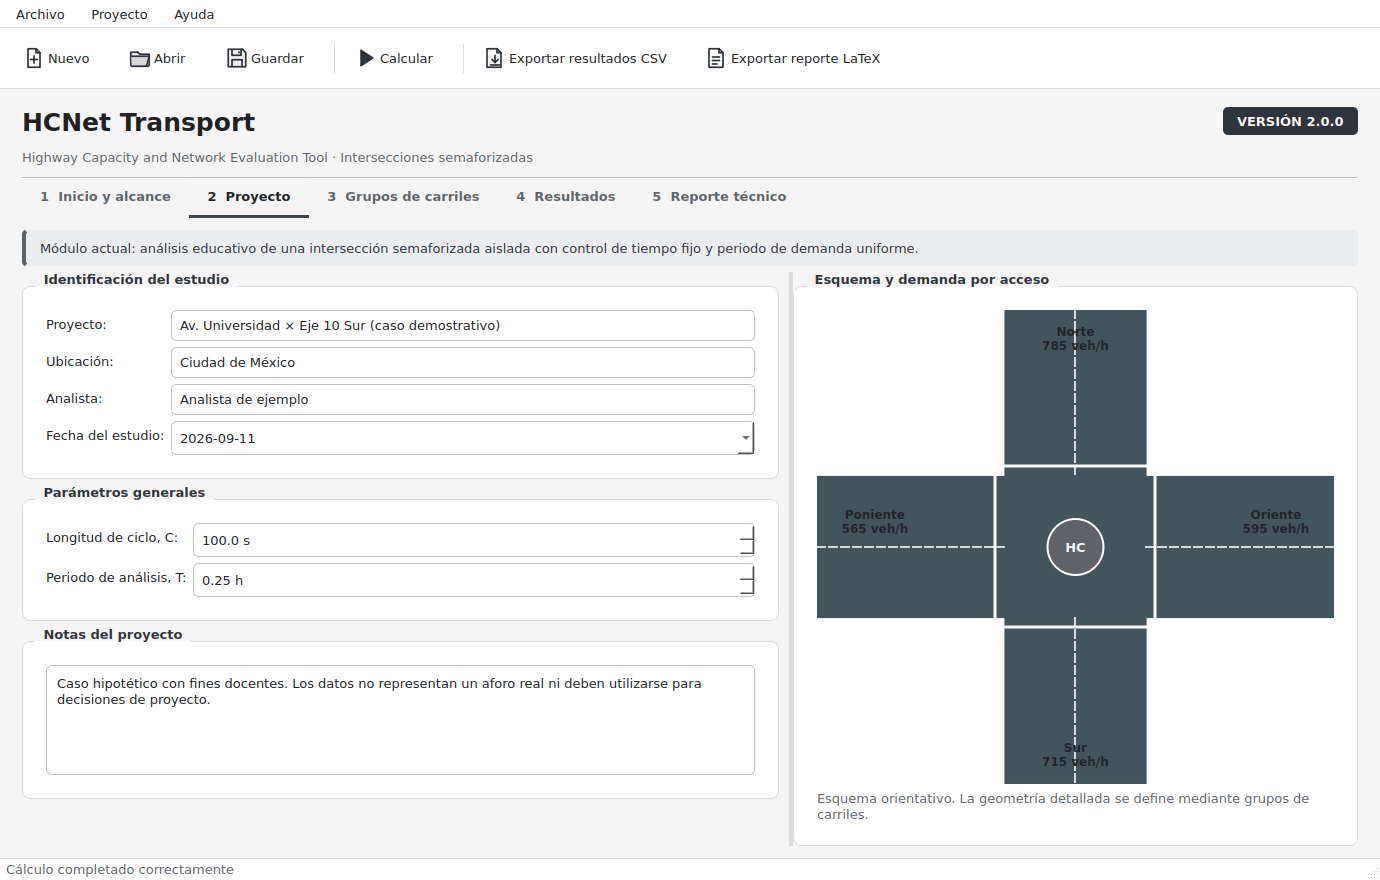
\includegraphics[width=0.98\textwidth]{02_proyecto.png}
  \caption{Identificación y parámetros comunes del proyecto.}
  \label{fig:proyecto}
\end{figure}

\begin{table}[H]
\centering
\caption{Campos del proyecto.}
\label{tab:campos-proyecto}
\begin{tabularx}{\textwidth}{@{}p{3.7cm}p{3.1cm}Y@{}}
\toprule
\rowcolor{hcPale}
\textbf{Campo} & \textbf{Formato} & \textbf{Uso} \\
\midrule
Nombre del proyecto & Texto & Identifica la intersección o alternativa analizada. \\
Ubicación & Texto & Ciudad, corredor, coordenadas o referencia espacial. \\
Analista & Texto & Aparece en el reporte LaTeX; es obligatorio para exportarlo. \\
Fecha del estudio & AAAA-MM-DD & Fecha de aforo o de análisis, según se documente. \\
Longitud de ciclo, $C$ & segundos & Ciclo común del plan semafórico; intervalo de
captura 1 a 600 s. HCNet advierte valores fuera de 30 a 240 s. \\
Periodo de análisis, $T$ & horas & Duración representada por la demanda; intervalo
de captura 0.05 a 4 h. Valores mayores a 1 h generan advertencia. \\
Notas & Texto libre & Registra fuentes, supuestos, escenario y observaciones. \\
\bottomrule
\end{tabularx}
\end{table}

\begin{tipbox}[Trazabilidad mínima del estudio]
Incluya en las notas: fuente y fecha de los aforos, intervalo de máxima demanda,
origen del plan semafórico, criterio para agrupar movimientos, versión del modelo
y toda modificación aplicada a factores por defecto.
\end{tipbox}

\section{Creación, apertura y guardado}

Los proyectos se almacenan como JSON UTF-8 con la extensión recomendada
\texttt{.hcnet.json}. El archivo contiene versión de esquema, versión de la
aplicación, datos generales y todos los grupos de carriles.\index{archivo de
proyecto}\index{JSON}

\begin{procedurebox}[Crear y guardar un proyecto]
\begin{enumerate}
  \item Seleccione \textbf{Archivo > Nuevo}.
  \item Complete los campos de identificación y parámetros temporales.
  \item Agregue por lo menos un grupo de carriles.
  \item Seleccione \textbf{Archivo > Guardar como}.
  \item Use un nombre que identifique ubicación, escenario y fecha, por ejemplo
        \texttt{universidad\_base\_2026.hcnet.json}.
\end{enumerate}
\end{procedurebox}

HCNet realiza una escritura atómica: primero crea un archivo temporal y después
reemplaza el destino. Esta estrategia reduce el riesgo de dejar un proyecto
parcialmente escrito si ocurre una interrupción.

% =============================================================================
\chapter{Definición de grupos de carriles}
% =============================================================================

\section{Unidad de análisis}

Un grupo de carriles reúne uno o varios carriles que operan con condiciones de
demanda, señalización y uso suficientemente homogéneas para ser analizados como
una unidad. La formación del grupo es una decisión de ingeniería previa al
cálculo. HCNet no asigna automáticamente movimientos a carriles compartidos.
\index{grupo de carriles}

\begin{figure}[H]
  \centering
  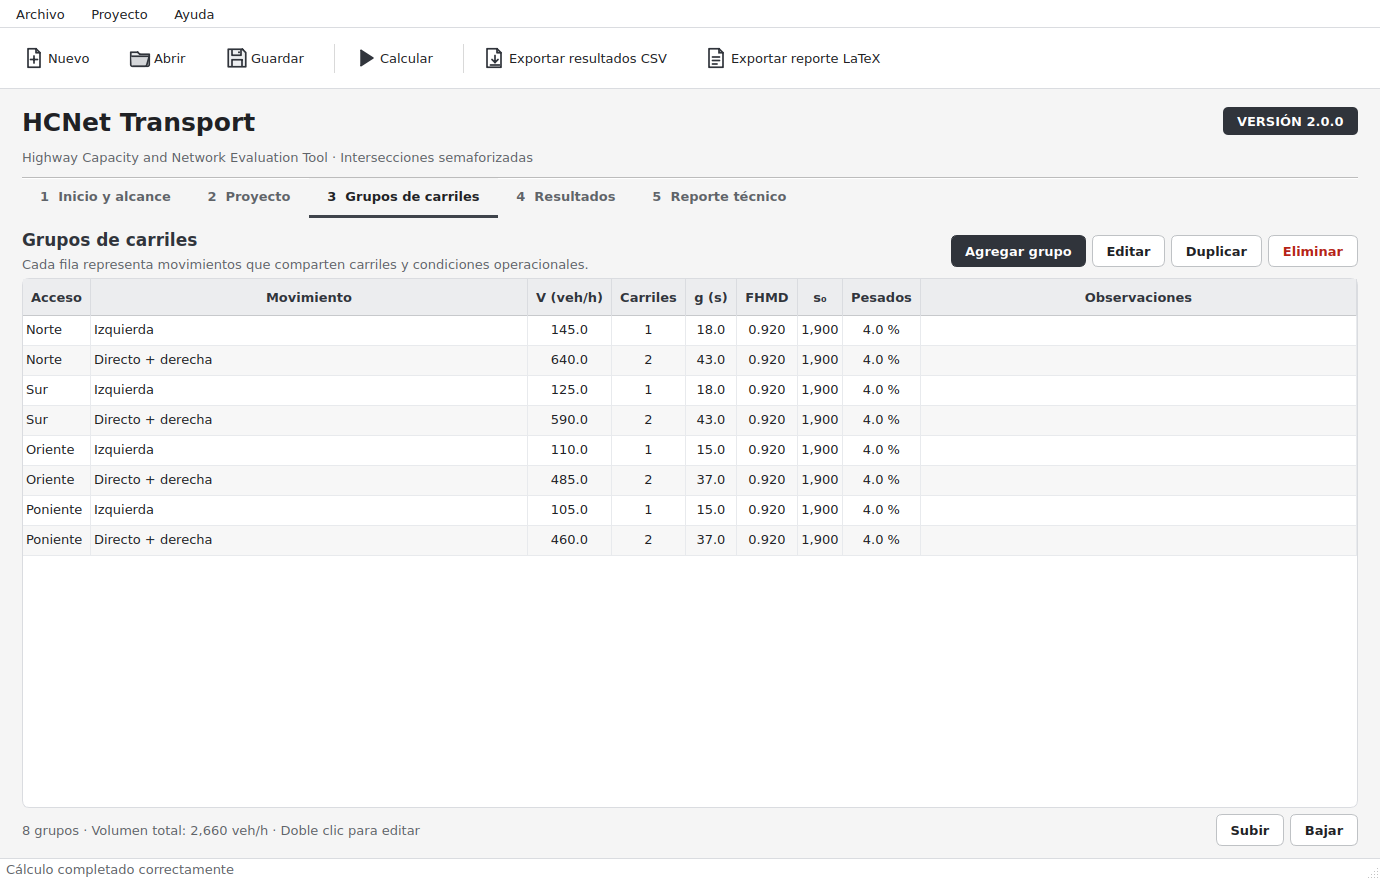
\includegraphics[width=0.98\textwidth]{03_grupos_carriles.png}
  \caption{Lista de grupos de carriles del caso demostrativo.}
  \label{fig:grupos}
\end{figure}

Los botones \textbf{Agregar}, \textbf{Editar}, \textbf{Duplicar} y
\textbf{Eliminar} administran la lista. Duplicar es útil cuando dos grupos
comparten gran parte de sus parámetros; después de duplicar, cambie acceso,
movimiento y cualquier dato que corresponda.

\section{Datos básicos}

\begin{figure}[H]
  \centering
  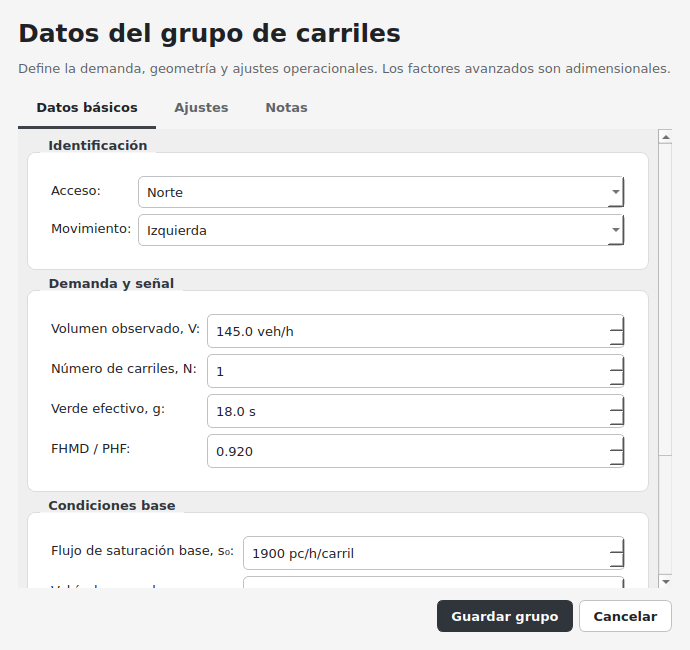
\includegraphics[width=0.74\textwidth]{04_grupo_datos_basicos.png}
  \caption{Captura de demanda, geometría y tiempo efectivo de un grupo.}
  \label{fig:grupo-basico}
\end{figure}

\begin{longtable}{@{}p{3.0cm}p{2.0cm}p{2.4cm}p{6.6cm}@{}}
\caption{Entradas básicas de un grupo de carriles.}\label{tab:entradas-basicas}\\
\toprule
\rowcolor{hcPale}
\textbf{Parámetro} & \textbf{Símbolo} & \textbf{Captura} & \textbf{Interpretación} \\
\midrule
\endfirsthead
\toprule
\rowcolor{hcPale}
\textbf{Parámetro} & \textbf{Símbolo} & \textbf{Captura} & \textbf{Interpretación} \\
\midrule
\endhead
Acceso & - & Texto & Identifica el ramal: Norte, Sur, Oriente, Poniente u
otra denominación definida por el analista. \\
Movimiento & - & Texto & Giro o combinación que integra el grupo. \\
Volumen & $V$ & 0 a 20,000 veh/h & Volumen horario observado o equivalente. \\
Carriles & $N$ & 1 a 12 & Número de carriles del grupo. \\
Verde efectivo & $g$ & 0.1 a 600 s & Tiempo efectivo disponible por ciclo;
debe ser menor que $C$. \\
Factor de hora de máxima demanda & FHMD & 0.01 a 1.00 & Convierte el volumen
horario en tasa de flujo durante el intervalo crítico. \\
Flujo de saturación base & $s_0$ & 500 a 3\,000 pc/h/carril & Valor base antes de
factores. HCNet advierte si está fuera de 1,500 a 2,200. \\
Vehículos pesados & $P_{HV}$ & 0 a 100\% & Participación porcentual de vehículos
pesados. \\
Equivalencia de pesados & $E_T$ & 1 a 5 & Equivalencia en automóviles de pasajero. \\
Ancho de carril & $w$ & 2.4 a 4.8 m & Ancho representativo del grupo. \\
Pendiente & $G$ & -10 a +10\% & Signo positivo para ascenso y negativo para descenso. \\
\bottomrule
\end{longtable}

\begin{warningbox}[Rango de captura y validez metodológica]
Un valor aceptado por el control de interfaz no es automáticamente válido para
todo contexto. Los intervalos de captura protegen la operación del programa; el
analista debe justificar la aplicabilidad metodológica de cada dato.
\end{warningbox}

\section{Factores y parámetros de demora}

\begin{figure}[H]
  \centering
  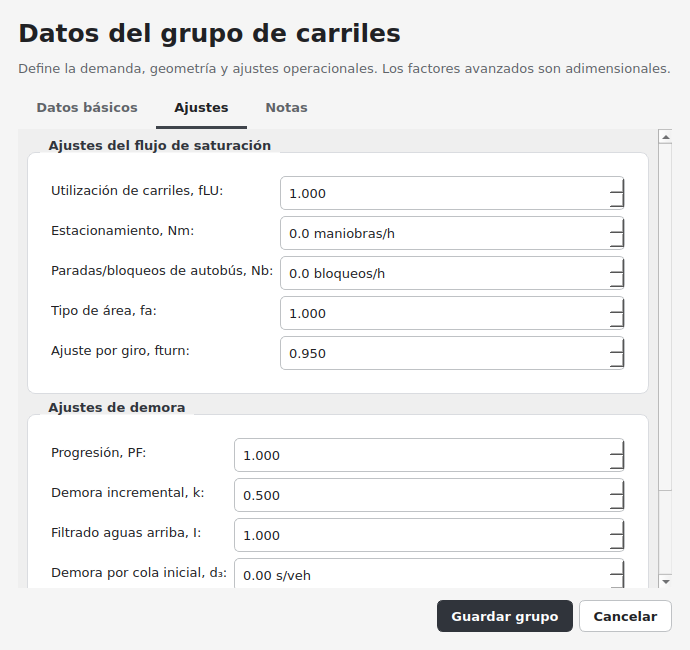
\includegraphics[width=0.74\textwidth]{05_grupo_ajustes.png}
  \caption{Factores de ajuste y parámetros de demora incremental.}
  \label{fig:grupo-ajustes}
\end{figure}

\begin{longtable}{@{}p{3.6cm}p{1.7cm}p{2.2cm}p{6.5cm}@{}}
\caption{Ajustes del grupo de carriles.}\label{tab:ajustes}\\
\toprule
\rowcolor{hcPale}
\textbf{Parámetro} & \textbf{Símbolo} & \textbf{Captura} & \textbf{Uso en HCNet} \\
\midrule
\endfirsthead
\toprule
\rowcolor{hcPale}
\textbf{Parámetro} & \textbf{Símbolo} & \textbf{Captura} & \textbf{Uso en HCNet} \\
\midrule
\endhead
Utilización de carriles & $f_{LU}$ & 0.05 a 1.50 & Factor suministrado por el usuario
para el flujo de saturación. \\
Maniobras de estacionamiento & $N_m$ & 0 a 1\,000/h & HCNet calcula $f_p$ a
partir de la frecuencia indicada. \\
Bloqueos de autobús & $N_b$ & 0 a 1\,000/h & HCNet calcula $f_{bb}$ a partir
de la frecuencia indicada. \\
Tipo de área & $f_a$ & 0.05 a 1.50 & Factor suministrado por el usuario. \\
Giro & $f_{turn}$ & 0.05 a 1.50 & Factor que representa efectos del movimiento. \\
Progresión & PF & 0.05 a 1.50 & Multiplica la componente de demora uniforme. \\
Demora incremental & $k$ & 0.01 a 1.50 & Parámetro de calibración de $d_2$. \\
Filtrado aguas arriba & $I$ & 0.01 a 1.50 & Representa el efecto de filtrado en $d_2$. \\
Demora por cola inicial & $d_3$ & 0 a 3\,600 s/veh & Componente suministrada por
el usuario; HCNet no la estima internamente. \\
\bottomrule
\end{longtable}

Los factores $f_w$, $f_{HV}$, $f_g$, $f_p$ y $f_{bb}$ son calculados por HCNet
con las expresiones descritas en el capítulo~\ref{chap:metodologia}. Los factores
$f_{LU}$, $f_a$ y $f_{turn}$, así como PF, $k$, $I$ y $d_3$, dependen de la
entrada del usuario.

\begin{tipbox}[Uso de valores por defecto]
El valor 1.0 significa ausencia de ajuste para $f_{LU}$, $f_a$, $f_{turn}$, PF e
$I$; no significa que se haya comprobado que la condición de campo sea neutra.
Conserve 1.0 solamente cuando exista una razón técnica documentada.
\end{tipbox}

% =============================================================================
\chapter{Cálculo y lectura de resultados}
% =============================================================================

\section{Ejecución del análisis}

Para calcular, seleccione \textbf{Proyecto > Calcular}, pulse el botón
\textbf{Calcular} en la barra de herramientas o presione F5. HCNet primero
sincroniza los controles, ejecuta la validación y detiene el proceso si encuentra
errores.

\begin{procedurebox}[Revisión antes de calcular]
\begin{enumerate}
  \item Confirme que $C$ y $T$ pertenecen al escenario estudiado.
  \item Compruebe que existe al menos un grupo y que no hay nombres ambiguos.
  \item Verifique $V$, $N$, $g$, FHMD, $s_0$, composición vehicular, ancho y
        pendiente.
  \item Revise todos los factores que no calcula HCNet.
  \item Documente el origen de PF, $k$, $I$ y $d_3$.
\end{enumerate}
\end{procedurebox}

\section{Resumen de la intersección}

\begin{figure}[H]
  \centering
  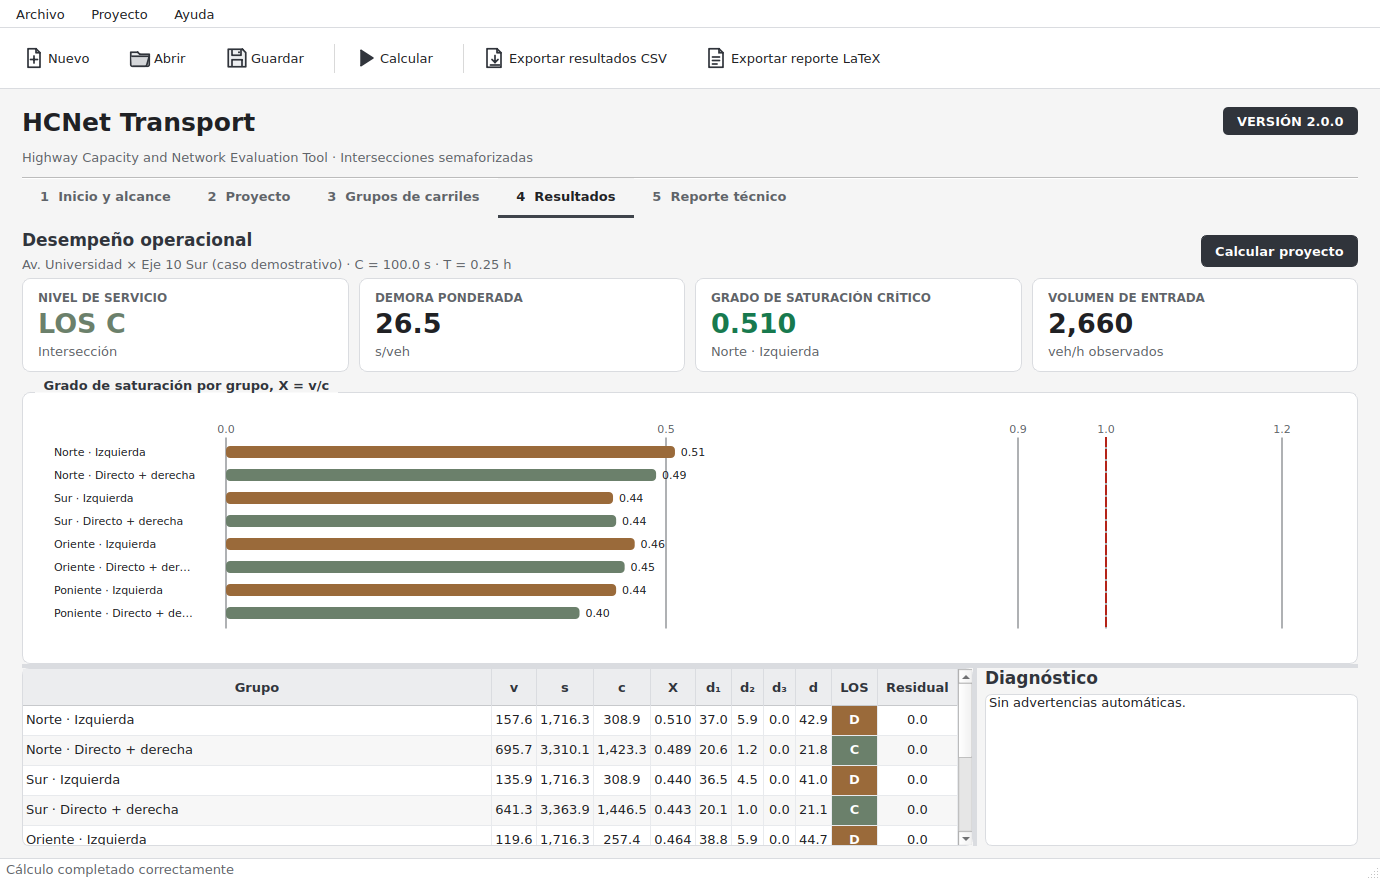
\includegraphics[width=0.98\textwidth]{06_resultados.png}
  \caption{Resumen, gráfica y tabla de resultados del caso demostrativo.}
  \label{fig:resultados}
\end{figure}

La franja superior de \textbf{Resultados} presenta:

\begin{itemize}
  \item \textbf{nivel de servicio de la intersección}: clasificación A a F basada
        en la demora ponderada;
  \item \textbf{demora ponderada}: promedio de demora de los grupos ponderado por
        la tasa de flujo ajustada;
  \item \textbf{$X$ crítico}: mayor grado de saturación entre los grupos;
  \item \textbf{volumen de entrada}: suma de volúmenes observados $V$;
  \item \textbf{grupo crítico}: grupo asociado con el mayor $X$.
\end{itemize}

\begin{keybox}[Dos medidas distintas]
La demora ponderada determina el nivel de servicio de la intersección. El máximo
$X$ identifica la condición de saturación más exigente. No deben interpretarse
como indicadores equivalentes: una demora global moderada puede coexistir con
un grupo de carriles cercano o superior a la capacidad.
\end{keybox}

\section{Resultados por grupo}

La tabla inferior contiene las variables indicadas en la
tabla~\ref{tab:salidas-grupo}. Al seleccionar una fila, la pestaña
\textbf{Reporte técnico} cambia a la memoria correspondiente.

\begin{table}[H]
\centering
\caption{Salidas principales por grupo de carriles.}
\label{tab:salidas-grupo}
\begin{tabularx}{\textwidth}{@{}p{3.4cm}p{2.4cm}Y@{}}
\toprule
\rowcolor{hcPale}
\textbf{Salida} & \textbf{Unidad} & \textbf{Interpretación} \\
\midrule
Flujo ajustado, $v$ & veh/h & Tasa crítica obtenida de $V/\mathrm{FHMD}$. \\
Flujo de saturación, $s$ & veh/h & Flujo base del grupo después de factores. \\
Capacidad, $c$ & veh/h & Producto de $s$ por la proporción $g/C$. \\
Grado de saturación, $X$ & adimensional & Cociente $v/c$. \\
Demora $d_1$ & s/veh & Componente uniforme ajustada por progresión. \\
Demora $d_2$ & s/veh & Componente incremental. \\
Demora $d_3$ & s/veh & Componente por cola inicial introducida por el usuario. \\
Demora de control, $d$ & s/veh & Suma de las tres componentes. \\
LOS & A a F & Nivel de servicio del grupo. \\
Llegadas en rojo & veh/ciclo & Estimación diagnóstica $v(C-g)/3600$. \\
Demanda residual & veh & Exceso diagnóstico $\max[0,(v-c)T]$. \\
\bottomrule
\end{tabularx}
\end{table}

\begin{warningbox}[Interpretación de sobresaturación]
Cuando $X>1$, HCNet asigna nivel de servicio F al grupo, aunque la demora calculada
quede debajo del umbral ordinario de F. Revise también demanda residual, periodo
de análisis y cola inicial; no limite la conclusión a una sola letra.
\end{warningbox}

% =============================================================================
\chapter{Memoria de cálculo y exportaciones}
% =============================================================================

\section{Reporte técnico en pantalla}

La pestaña \textbf{Reporte técnico} desglosa el grupo seleccionado: demanda
ajustada, factores, flujo de saturación, capacidad, $X$, componentes de demora,
nivel de servicio e indicadores diagnósticos.

\begin{figure}[H]
  \centering
  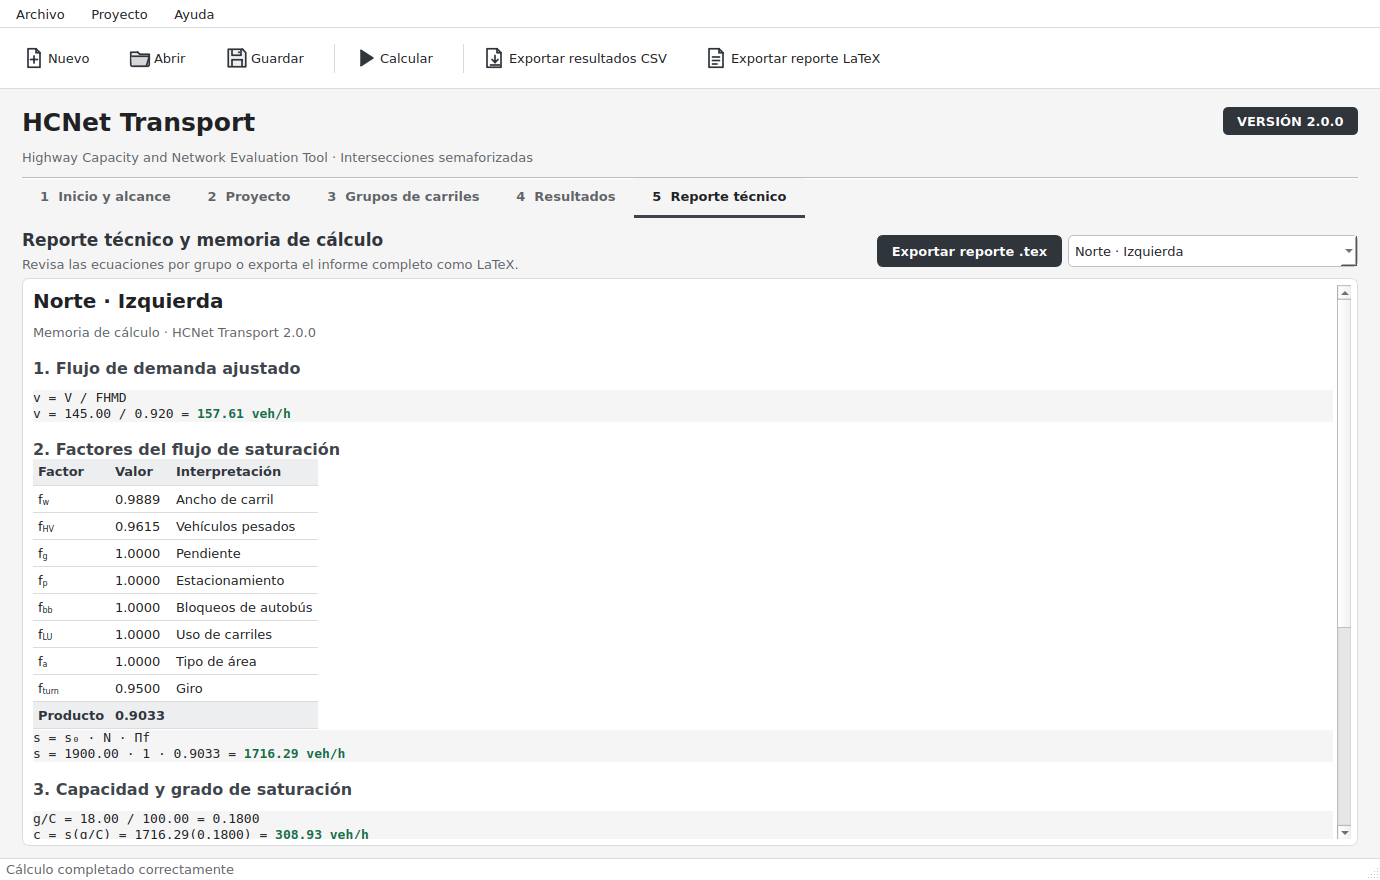
\includegraphics[width=0.98\textwidth]{07_reporte_tecnico.png}
  \caption{Memoria de cálculo trazable para el grupo seleccionado.}
  \label{fig:reporte}
\end{figure}

Esta vista permite auditar la secuencia numérica sin abandonar la aplicación. La
memoria se actualiza al seleccionar otro renglón en \textbf{Resultados}.

\section{Exportación del reporte LaTeX}

\begin{procedurebox}[Generar el archivo \texttt{.tex}]
\begin{enumerate}
  \item Complete el campo \textbf{Analista} en la pestaña \textbf{Proyecto}.
  \item Ejecute el cálculo y atienda los diagnósticos relevantes.
  \item Seleccione \textbf{Archivo > Exportar reporte LaTeX} o use
        Ctrl+Mayús+E.
  \item Elija la carpeta y el nombre del archivo \texttt{.tex}.
  \item Abra el archivo para revisión o compílelo con PDFLaTeX.
\end{enumerate}
\end{procedurebox}

El reporte generado es autocontenido e incluye portada, identificación del
proyecto, nombre del analista, fecha, versión del software, licencia, resumen de
la intersección, resultados por grupo, memoria numérica, diagnósticos y aviso de
alcance.

Para compilarlo en una terminal con una distribución LaTeX instalada:

\begin{lstlisting}
pdflatex nombre_del_reporte.tex
pdflatex nombre_del_reporte.tex
\end{lstlisting}

\begin{warningbox}
La exportación LaTeX se bloquea si el nombre del analista está vacío. Este control
es intencional: un reporte técnico debe conservar la responsabilidad e identidad
de quien efectuó y revisó el análisis.
\end{warningbox}

\section{Exportación CSV}

Seleccione \textbf{Archivo > Exportar resultados CSV} o Ctrl+E. El archivo usa
codificación UTF-8 con marca BOM para mejorar la apertura en hojas de cálculo y
contiene una fila por grupo. Incluye identificación, demanda, capacidad, demora,
nivel de servicio, indicadores diagnósticos y factores de ajuste.\index{CSV}

\begin{tipbox}[Control de versiones del estudio]
Guarde juntos el proyecto \texttt{.hcnet.json}, el CSV, el reporte \texttt{.tex}
y el PDF compilado. Evite sobrescribir escenarios; use sufijos como
\texttt{base}, \texttt{alternativa-a} y \texttt{sensibilidad-pf}.
\end{tipbox}

% =============================================================================
\chapter{Fundamento metodológico implementado}
\label{chap:metodologia}
% =============================================================================

\section{Naturaleza del modelo}

HCNet implementa un flujo de trabajo transparente, inspirado en conceptos del
análisis operacional de intersecciones semaforizadas del \textit{Highway Capacity
Manual}, séptima edición \cite{hcm2022}. Las expresiones de este capítulo describen
el comportamiento exacto de la versión \softwareVersion; por ello permiten
reproducir y auditar el resultado del software.\index{HCM}

\begin{limitbox}[Alcance de las ecuaciones]
La implementación es deliberadamente acotada y educativa. No representa todos
los procedimientos, tablas, casos especiales ni calibraciones del HCM. Consulte
una fuente autorizada antes de transferir estas ecuaciones a un contexto distinto
del descrito en este manual.
\end{limitbox}

\section{Tasa de flujo de demanda}

Para cada grupo, HCNet convierte el volumen horario $V$ en tasa de flujo ajustada:

\begin{equationbox}
\begin{equation}
v=\frac{V}{\mathrm{FHMD}},
\label{eq:v}
\end{equation}
donde $v$ y $V$ se expresan en veh/h y $0<\mathrm{FHMD}\leq 1$.
\end{equationbox}

\section{Factores calculados por el software}

Los porcentajes se convierten a fracción antes de operar. HCNet calcula:

\begin{align}
f_w &= \operatorname{lim}_{[0.80,1.20]}
       \left(1+\frac{w-3.6}{9}\right), \\
f_{HV} &= \frac{1}{1+P_{HV}(E_T-1)}, \\
f_g &= \operatorname{lim}_{[0.80,1.20]}
       \left(1-\frac{G}{200}\right).
\end{align}

La función $\operatorname{lim}_{[a,b]}$ restringe el resultado al intervalo
$[a,b]$. Para estacionamiento:

\begin{equation}
f_p=
\begin{cases}
1, & N_m=0,\\
\operatorname{lim}_{[0.05,1.00]}
\left(\dfrac{N-0.1-18(N_m/3600)}{N}\right), & N_m>0.
\end{cases}
\end{equation}

Para bloqueos de autobús:

\begin{equation}
f_{bb}=\operatorname{lim}_{[0.05,1.00]}
\left(\frac{N-14.4(N_b/3600)}{N}\right).
\end{equation}

\section{Flujo de saturación, capacidad y saturación}

El flujo de saturación ajustado es:

\begin{equationbox}
\begin{align}
s &= s_0N f_w f_{HV}f_gf_pf_{bb}f_{LU}f_af_{turn}, \\
c &= s\left(\frac{g}{C}\right), \\
X &= \frac{v}{c}.
\end{align}
\end{equationbox}

$s_0$ se expresa en pc/h/carril; $N$ es el número de carriles; $g/C$ es la
proporción efectiva de verde. En la salida, $s$ y $c$ se muestran en veh/h como
tasas equivalentes del grupo.

\section{Demora de control}

La componente uniforme se calcula como:

\begin{equation}
d_1=\frac{0.5C(1-g/C)^2}{1-\min(1,X)(g/C)}\,PF.
\end{equation}

La componente incremental es:

\begin{equation}
d_2=900T\left[(X-1)+
\sqrt{(X-1)^2+\frac{8kIX}{cT}}\right],
\end{equation}

y HCNet restringe cualquier residuo numérico negativo de $d_2$ a cero. La demora
total es:

\begin{equationbox}
\begin{equation}
d=d_1+d_2+d_3.
\end{equation}
$d_3$ no se estima: el usuario debe introducir una demora por cola inicial
coherente con su método y escenario.
\end{equationbox}

\section{Nivel de servicio}

La tabla~\ref{tab:los} contiene los umbrales programados para grupos de carriles
y para la demora ponderada de la intersección.

\begin{table}[H]
\centering
\caption{Umbrales de nivel de servicio basados en demora de control.}
\label{tab:los}
\begin{tabular}{@{}C{2.5cm}C{5.0cm}@{}}
\toprule
\rowcolor{hcPale}
\textbf{Nivel} & \textbf{Demora $d$ (s/veh)} \\
\midrule
A & $d\leq 10$ \\
B & $10<d\leq 20$ \\
C & $20<d\leq 35$ \\
D & $35<d\leq 55$ \\
E & $55<d\leq 80$ \\
F & $d>80$ \\
\bottomrule
\end{tabular}
\end{table}

Para un grupo, $X>1$ fuerza LOS F. Para la intersección, HCNet clasifica la
demora ponderada sin forzar F a partir del $X$ crítico; ambos indicadores se
presentan de forma separada.

\section{Agregación e indicadores diagnósticos}

La demora de la intersección se pondera mediante:

\begin{equation}
d_I=\frac{\sum_i v_i d_i}{\sum_i v_i}.
\end{equation}

El grupo crítico es el que presenta el máximo $X_i$. HCNet calcula además:

\begin{align}
A_r &= \frac{v(C-g)}{3600}, \\
D_r &= \max\left[0,(v-c)T\right],
\end{align}

donde $A_r$ son llegadas estimadas durante el rojo en veh/ciclo y $D_r$ es una
demanda residual diagnóstica en vehículos.

% =============================================================================
\chapter{Caso demostrativo reproducible}
% =============================================================================

\section{Objetivo}

El caso integrado permite comprobar la operación de la interfaz y obtener una
referencia numérica. No representa una calibración universal ni un proyecto real.
Para cargarlo seleccione \textbf{Proyecto > Cargar caso demostrativo} y después
presione F5.

\section{Identificación y demanda}

\begin{table}[H]
\centering
\caption{Parámetros generales del caso demostrativo.}
\label{tab:demo-general}
\begin{tabularx}{\textwidth}{@{}p{4.4cm}Y@{}}
\toprule
\rowcolor{hcPale}
\textbf{Elemento} & \textbf{Valor} \\
\midrule
Proyecto & Av. Universidad $\times$ Eje 10 Sur (caso demostrativo) \\
Ubicación & Ciudad de México \\
Longitud de ciclo, $C$ & 100 s \\
Periodo de análisis, $T$ & 0.25 h \\
Número de grupos & 8 \\
Volumen total observado & 2,660 veh/h \\
\bottomrule
\end{tabularx}
\end{table}

\begin{table}[H]
\centering
\caption{Volumen, carriles y verde del caso demostrativo.}
\label{tab:demo-entradas}
\small
\begin{tabular}{@{}lrrrrrr@{}}
\toprule
\rowcolor{hcPale}
\textbf{Grupo} & \textbf{$V$} & \textbf{$N$} & \textbf{$g$} & \textbf{FHMD}
& \textbf{$s_0$} & \textbf{$P_{HV}$} \\
 & veh/h & & s & & pc/h/carril & \% \\
\midrule
Norte - Izquierda & 145 & 1 & 18 & 0.92 & 1900 & 4 \\
Norte - Directo+derecha & 640 & 2 & 43 & 0.92 & 1900 & 4 \\
Sur - Izquierda & 125 & 1 & 18 & 0.92 & 1900 & 4 \\
Sur - Directo+derecha & 590 & 2 & 43 & 0.92 & 1900 & 3 \\
Oriente - Izquierda & 110 & 1 & 15 & 0.92 & 1900 & 4 \\
Oriente - Directo+derecha & 485 & 2 & 37 & 0.92 & 1900 & 3 \\
Poniente - Izquierda & 105 & 1 & 15 & 0.92 & 1900 & 4 \\
Poniente - Directo+derecha & 460 & 2 & 37 & 0.92 & 1900 & 3 \\
\bottomrule
\end{tabular}
\end{table}

\section{Resultados de referencia}

Al calcular con la versión \softwareVersion\ se deben obtener, salvo diferencias
de redondeo de presentación, los valores de la tabla~\ref{tab:demo-salidas}.

\begin{table}[H]
\centering
\caption{Resultados de referencia por grupo.}
\label{tab:demo-salidas}
\small
\begin{tabular}{@{}lrrrrr@{}}
\toprule
\rowcolor{hcPale}
\textbf{Grupo} & \textbf{$v$} & \textbf{$c$} & \textbf{$X$} & \textbf{$d$} & \textbf{LOS} \\
 & veh/h & veh/h & & s/veh & \\
\midrule
Norte - Izquierda & 157.61 & 308.93 & 0.510 & 42.93 & D \\
Norte - Directo+derecha & 695.65 & 1423.35 & 0.489 & 21.77 & C \\
Sur - Izquierda & 135.87 & 308.93 & 0.440 & 41.00 & D \\
Sur - Directo+derecha & 641.30 & 1446.49 & 0.443 & 21.06 & C \\
Oriente - Izquierda & 119.57 & 257.44 & 0.464 & 44.75 & D \\
Oriente - Directo+derecha & 527.17 & 1163.75 & 0.453 & 25.12 & C \\
Poniente - Izquierda & 114.13 & 257.44 & 0.443 & 44.15 & D \\
Poniente - Directo+derecha & 500.00 & 1244.66 & 0.402 & 24.28 & C \\
\bottomrule
\end{tabular}
\end{table}

\begin{keybox}[Resultado consolidado de referencia]
La demora ponderada de la intersección es 26.55 s/veh y corresponde a LOS C. El
grado de saturación crítico es 0.510 y pertenece al grupo Norte - Izquierda. El
caso no produce advertencias automáticas ni demanda residual.
\end{keybox}

\section{Interpretación técnica}

El LOS C global no implica que todos los grupos operen en C: los cuatro grupos de
giro izquierdo presentan LOS D. El grupo crítico se identifica por el mayor $X$,
pero la mayor demora corresponde al grupo Oriente - Izquierda. Esta diferencia
confirma la necesidad de revisar simultáneamente capacidad, saturación y demora.

\begin{tipbox}[Ensayo de sensibilidad]
Duplique el proyecto y modifique un parámetro a la vez, por ejemplo $g$, FHMD o
PF. Compare CSV y reporte LaTeX entre escenarios. No mezcle en una misma corrida
cambios de demanda, geometría y control si desea atribuir el efecto a una causa.
\end{tipbox}

% =============================================================================
\chapter{Validación y solución de problemas}
% =============================================================================

\section{Errores que impiden calcular}

HCNet bloquea el análisis cuando detecta datos no finitos, ciclo o periodo no
positivos, ausencia de grupos, acceso o movimiento vacío, volumen negativo,
menos de un carril, $g\leq0$, $g\geq C$, FHMD fuera de $(0,1]$, $s_0\leq0$,
porcentaje de pesados fuera de 0 a 100, $E_T<1$, ancho fuera de 2.4 a 4.8 m,
pendiente fuera de -10 a 10\%, factores no positivos, maniobras o bloqueos
negativos, o $d_3<0$.

\section{Advertencias que requieren criterio}

El cálculo puede continuar cuando el nombre del proyecto está vacío, $C$ queda
fuera de 30 a 240 s, $T>1$ h, $s_0$ queda fuera de 1\,500 a 2\,200 pc/h/carril o
algún factor supera 1.5. Una advertencia no invalida automáticamente el análisis,
pero debe ser revisada y documentada.\index{validación}\index{advertencia}

\begin{table}[H]
\centering
\caption{Lista de control de calidad antes de emitir un reporte.}
\label{tab:control-calidad}
\begin{tabularx}{\textwidth}{@{}C{1.2cm}Y@{}}
\toprule
\rowcolor{hcPale}
\textbf{Núm.} & \textbf{Comprobación} \\
\midrule
1 & El archivo corresponde al escenario, fecha y versión identificados. \\
2 & La suma de movimientos es coherente con el volumen de entrada documentado. \\
3 & Los grupos reflejan la canalización y uso de carriles observados. \\
4 & El verde efectivo, el ciclo y la progresión corresponden al mismo plan. \\
5 & Los factores no calculados por HCNet tienen fuente o justificación. \\
6 & Las advertencias automáticas fueron resueltas o explicadas. \\
7 & Se revisaron $X$, $d$, LOS y demanda residual por grupo, no solo el resumen. \\
8 & El reporte identifica al analista y conserva archivos de entrada y salida. \\
\bottomrule
\end{tabularx}
\end{table}

\section{Problemas frecuentes en Linux}

\begin{longtable}{@{}p{4.4cm}p{5.0cm}p{4.9cm}@{}}
\caption{Diagnóstico básico de ejecución.}\label{tab:problemas}\\
\toprule
\rowcolor{hcPale}
\textbf{Síntoma} & \textbf{Causa probable} & \textbf{Acción recomendada} \\
\midrule
\endfirsthead
\toprule
\rowcolor{hcPale}
\textbf{Síntoma} & \textbf{Causa probable} & \textbf{Acción recomendada} \\
\midrule
\endhead
\texttt{hcnet: command not found} & Entorno virtual inactivo o paquete no
instalado. & Active \texttt{.venv} y repita \texttt{pip install -e ".[dev]"}. \\
Error de módulo PySide6 & Dependencias instaladas fuera del entorno o instalación
incompleta. & Verifique \texttt{which python} y reinstale dentro de \texttt{.venv}. \\
Error del complemento Qt/XCB & Falta una biblioteca de escritorio. & En Ubuntu o
Debian instale \texttt{libxcb-cursor0}; revise el mensaje de Qt para dependencias
adicionales de su distribución. \\
No se abre una ventana & Sesión sin servidor gráfico o variable de pantalla no
disponible. & Ejecute desde una sesión gráfica local compatible. \\
Proyecto rechazado al abrir & JSON inválido, tipo de dato incorrecto o esquema más
reciente. & No edite a ciegas; conserve una copia, valide el JSON y actualice HCNet
si el mensaje indica versión futura. \\
No se puede exportar \texttt{.tex} & Analista vacío o resultados no calculados. &
Complete el analista y ejecute F5 antes de exportar. \\
\bottomrule
\end{longtable}

\section{Actualización del código}

Antes de actualizar, guarde una copia de los proyectos. Desde el repositorio:

\begin{lstlisting}
cd ~/hcnet-transport
git pull --ff-only
source .venv/bin/activate
python -m pip install -e ".[dev]"
pytest
\end{lstlisting}

Revise \texttt{CHANGELOG.md} para identificar cambios de versión y posibles
modificaciones de resultados.

% =============================================================================
\appendix
\chapter{Referencia rápida}
% =============================================================================

\section{Atajos de teclado}

\begin{tabularx}{\textwidth}{@{}p{4.0cm}Y@{}}
\toprule
\rowcolor{hcPale}
\textbf{Atajo} & \textbf{Acción} \\
\midrule
Ctrl+N & Nuevo proyecto \\
Ctrl+O & Abrir proyecto \\
Ctrl+S & Guardar \\
Ctrl+Mayús+S & Guardar como \\
Ctrl+E & Exportar resultados CSV \\
Ctrl+Mayús+E & Exportar reporte LaTeX \\
F5 & Calcular \\
Ctrl+Q & Salir \\
\bottomrule
\end{tabularx}

\section{Archivos producidos}

\begin{tabularx}{\textwidth}{@{}p{4.0cm}Y@{}}
\toprule
\rowcolor{hcPale}
\textbf{Extensión} & \textbf{Contenido} \\
\midrule
\texttt{.hcnet.json} & Proyecto editable con parámetros y grupos de carriles. \\
\texttt{.csv} & Resultados tabulares para análisis posterior. \\
\texttt{.tex} & Memoria técnica en código fuente LaTeX. \\
\texttt{.pdf} & Producto opcional obtenido al compilar el archivo LaTeX. \\
\bottomrule
\end{tabularx}

\section{Columnas del CSV}

El archivo CSV contiene las siguientes 25 columnas, en este orden:

\begin{center}
\begingroup
\scriptsize
\renewcommand{\arraystretch}{0.92}
\begin{tabular}{@{}r p{6.3cm} r p{6.0cm}@{}}
\toprule
\rowcolor{hcPale}
\textbf{Núm.} & \textbf{Columna} & \textbf{Núm.} & \textbf{Columna} \\
\midrule
1 & \texttt{proyecto} & 14 & \texttt{nivel\_servicio} \\
2 & \texttt{ubicacion} & 15 & \texttt{llegadas\_en\_rojo\_veh\_ciclo} \\
3 & \texttt{acceso} & 16 & \texttt{demanda\_residual\_veh} \\
4 & \texttt{movimiento} & 17 & \texttt{fw} \\
5 & \texttt{volumen\_veh\_h} & 18 & \texttt{fHV} \\
6 & \texttt{flujo\_ajustado\_veh\_h} & 19 & \texttt{fg} \\
7 & \texttt{flujo\_saturacion\_veh\_h} & 20 & \texttt{fp} \\
8 & \texttt{capacidad\_veh\_h} & 21 & \texttt{fbb} \\
9 & \texttt{grado\_saturacion\_X} & 22 & \texttt{fLU} \\
10 & \texttt{demora\_uniforme\_d1\_s\_veh} & 23 & \texttt{fa} \\
11 & \texttt{demora\_incremental\_d2\_s\_veh} & 24 & \texttt{fturn} \\
12 & \texttt{demora\_cola\_inicial\_d3\_s\_veh} & 25 & \texttt{producto\_factores} \\
13 & \texttt{demora\_control\_s\_veh} & & \\
\bottomrule
\end{tabular}
\endgroup
\end{center}

% =============================================================================
\chapter{Glosario de símbolos y términos}
% =============================================================================

\begin{longtable}{@{}p{2.5cm}p{4.2cm}p{7.3cm}@{}}
\caption{Símbolos principales.}\label{tab:simbolos}\\
\toprule
\rowcolor{hcPale}
\textbf{Símbolo} & \textbf{Unidad} & \textbf{Definición} \\
\midrule
\endfirsthead
\toprule
\rowcolor{hcPale}
\textbf{Símbolo} & \textbf{Unidad} & \textbf{Definición} \\
\midrule
\endhead
$V$ & veh/h & Volumen horario observado. \\
$v$ & veh/h & Tasa de flujo de demanda ajustada por FHMD. \\
$C$ & s & Longitud del ciclo semafórico. \\
$g$ & s & Tiempo verde efectivo del grupo. \\
$T$ & h & Periodo de análisis. \\
$s_0$ & pc/h/carril & Flujo de saturación base. \\
$s$ & veh/h & Flujo de saturación ajustado del grupo. \\
$c$ & veh/h & Capacidad del grupo. \\
$X$ & - & Grado de saturación $v/c$. \\
$d_1$ & s/veh & Demora uniforme. \\
$d_2$ & s/veh & Demora incremental. \\
$d_3$ & s/veh & Demora por cola inicial suministrada por el usuario. \\
$d$ & s/veh & Demora de control total. \\
FHMD & - & Factor de hora de máxima demanda. \\
LOS & A a F & Nivel de servicio, por sus siglas en inglés. \\
PF & - & Factor de ajuste por progresión. \\
$k$ & - & Factor de demora incremental. \\
$I$ & - & Factor de filtrado aguas arriba. \\
\bottomrule
\end{longtable}

\section*{Términos}

\textbf{Capacidad.} Tasa máxima de servicio estimada para el grupo bajo las
condiciones representadas.\index{capacidad}

\textbf{Demanda residual.} Exceso diagnóstico de demanda durante $T$ cuando
$v>c$; no equivale a cola percentil 95.\index{demanda residual}

\textbf{Demora de control.} Incremento de tiempo asociado con la operación del
control, expresado por vehículo.\index{demora de control}

\textbf{Grupo de carriles.} Unidad de análisis formada por carriles con operación
suficientemente homogénea.\index{grupo de carriles}

\textbf{Nivel de servicio.} Clasificación cualitativa A a F asociada en HCNet con
la demora de control y, para grupos sobresaturados, con $X>1$.\index{nivel de servicio}

\textbf{Proyecto.} Conjunto de identificación, parámetros comunes, grupos de
carriles y notas almacenado por HCNet.\index{proyecto}

% =============================================================================
\clearpage
\phantomsection
\addcontentsline{toc}{chapter}{Referencias}
\begin{thebibliography}{9}

\bibitem{hcm2022}
Transportation Research Board.
\textit{Highway Capacity Manual: A Guide for Multimodal Mobility Analysis}.
Seventh Edition. The National Academies Press, Washington, D.C., 2022.

\bibitem{trb-hcm}
Transportation Research Board.
\textit{Highway Capacity Manual}. Información editorial y recursos oficiales.
\url{https://www.trb.org/Main/Blurbs/182050.aspx}.

\bibitem{hcnet-repo}
Benítez García, Héctor Alonso.
\textit{HCNet Transport}. Código fuente, metodología, historial de cambios y
archivo de citación. Versión \softwareVersion.
\url{\repositoryURL}.

\end{thebibliography}

\clearpage
\phantomsection
\addcontentsline{toc}{chapter}{Índice alfabético}
\printindex

\end{document}
